\section{AHTR One-Third Assembly Optimization Results Discussion}
\label{sec:assem-discussion}
Chapter \ref{chap:ahtr-plank-opt-results} characterized the \gls{AHTR} plank model's 
driving factors for each reactor optimization objective and their relationship with 
one another. 
This section utilizes the previous \gls{AHTR} plank characterizations and conducts 
a deep-dive to verify if the same reactor optimization objective driving factors apply 
to the \gls{AHTR} one-third assembly model. 
I also analyze how their combined effects result in the optimal reactor models found by 
the multi-objective optimization simulations. 

\subsection{Discussion: Minimize $PF_{total}$ Objective}
\label{sec:assem-discussion-pf}
\paragraph{Simulation a-1a}
In Section \ref{sec:assem-1-obj-pf}'s simulation a-1a, I conducted a single-objective 
optimization simulation to minimize the one-third assembly's total fuel packing fraction 
($PF_{total}$) by varying $PF_{total}$ and TRISO distribution. 
In simulation a-1a, \gls{ROLLO} found that an \gls{AHTR} one-third assembly model with 
the most-minimized $PF_{total}$ has $PF_{total}= 0.0559$ and an oscillating TRISO distribution 
along the x-axis (Figure \ref{fig:assem-obj-1-pf-final}).

Section \ref{sec:plank-discussion-pf} concluded that for the \gls{AHTR} plank model, 
the minimize $PF_{total}$ objective is driven by maximizing the total fission reaction 
rates. 
I ran a simulation for constant $PF_{total} = 0.0559$ TRISO distribution and compared its 
fission reaction rate with the oscillating TRISO distribution that most-minimized 
$PF_{total}$. 
Figure \ref{fig:assem-0.0559-comparison} shows the TRISO distributions for the two 
compared simulations: Figure \ref{fig:assem-obj-1-pf-final}'s most-minimized $PF_{total}$ 
and the constant $PF_{total} = 0.0559$. 
\begin{figure}[htbp!]
    \centering
    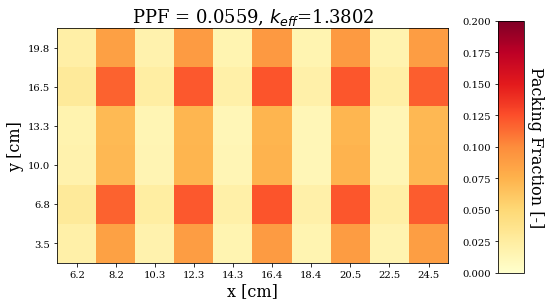
\includegraphics[width=0.49\linewidth]{assem-0.0559-most-minimized.png} 
    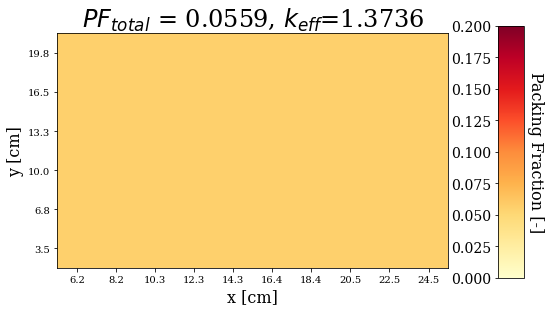
\includegraphics[width=0.49\linewidth]{assem-0.0559-flat.png} 
    \caption{Simulation a-1a's most-minimized $PF_{total}$ TRISO distribution 
    (oscillating TRISO distribution) from Figure \ref{fig:assem-obj-1-pf} (left) and the 
    constant $PF_{total} = 0.0559$ TRISO distribution (right).}
    \label{fig:assem-0.0559-comparison}
\end{figure}
The reactor model with the most-minimized $PF_{total}$ has $k_{eff}=1.3802$ and 
the reactor model with constant TRISO distribution has $k_{eff}=1.3736$.

Table \ref{tab:a-1a-fission-comparison} compares the total fission reaction rate 
(OpenMC's \texttt{fission} tally) between the most-minimized $PF_{total}$ TRISO 
distribution and a constant $PF_{total} = 0.0559$ TRISO distribution (both shown in 
Figure \ref{fig:assem-0.0559-comparison}).
\begin{table}[htbp!]
    \centering
    \onehalfspacing
    \caption{Total fission reaction rate comparison between simulation a-1a's 
    most-minimized $PF_{total}$ TRISO distribution and a constant $PF_{total} = 0.0559$ 
    TRISO distribution. Both distributions shown in Figure 
    \ref{fig:assem-0.0559-comparison}.}
	\label{tab:a-1a-fission-comparison}
    \footnotesize
    \begin{tabular}{p{1.5cm}lp{3.7cm}p{4cm}p{2.5cm}}
    \hline
    \textbf{Energy Group} & 
    \textbf{$\%$ of Total} &
    \textbf{Most-minimized $PF_{total}$ Fission \newline [reactions/src]} & 
    \textbf{Flat $PF_{total}$ Fission [reactions/src]} & 
    \textbf{$\%$ Fission \newline Difference}\\
    \hline 
    1 & 00.28 & 0.00165 & 0.00162 & \Plus2.01 \\
    2 & 01.56 & 0.00886 & 0.00884 & \Plus0.21 \\
    3 & 01.51 & 0.00854 & 0.00852 & \Plus0.23 \\
    4 & 96.63 & 0.54813 & 0.54465 & \Plus0.63 \\
    Total & - & 0.52998 & 0.52656 & \Plus0.65 \\
    \hline
    \end{tabular}
\end{table}
The most-minimized $PF_{total}$ TRISO distribution has $0.65\%$ higher  
\texttt{fission} (total fission reaction rate) than the constant 
$PF_{total} = 0.0559$ TRISO distribution, explaining why the oscillating TRISO 
distribution enabled a 650pcm higher $k_{eff}$ for the same $PF_{total}$ compared to the 
constant TRISO distribution. 

\paragraph{Simulation a-1d}
In Section \ref{sec:assem-1-obj-pf}'s simulation a-1d, I conducted a single-objective 
optimization simulation to minimize total fuel packing fraction ($PF_{total}$) by 
varying $PF_{total}$ and coolant channel shape. 
In simulation a-1d, \gls{ROLLO} found that there is no correlation 
between $PF_{total}$ and coolant channel shape (demonstrated in Figure 
\ref{fig:a-1d}). 

\paragraph{Summary}
I verified that the minimize $PF_{total}$ objective for the \gls{AHTR} one-third assembly 
model is also driven by maximizing the total fission reaction rates. 
The minimize $PF_{total}$ objective has correlations with the following input parameters: 
$PF_{total}$ and TRISO packing fraction distribution. 
The objective has no correlation with coolant channel shape input parameter. 

\subsection{Discussion: Minimize $T_{max}$ Objective}
\label{sec:assem-discussion-temp}
\paragraph{Simulation a-1b}
In Section \ref{sec:assem-1-obj-temp}'s simulation a-1b, I conducted a single-objective 
optimization simulation to minimize the one-third assembly's maximum temperature 
($T_{max}$) by varying TRISO distribution. 
In simulation a-1b, \gls{ROLLO} found that an \gls{AHTR} one-third assembly model with 
an almost constant TRISO distribution most-minimized $T_{max}$ 
(Figure \ref{fig:assem-obj-1-temp-final}).

\paragraph{Simulation a-1e}
In Section \ref{sec:assem-1-obj-temp}'s simulation a-1e, I conducted a single-objective 
optimization simulation to minimize the one-third assembly's maximum temperature 
($T_{max}$) by varying coolant channel shape. 
In simulation a-1e, \gls{ROLLO} found that there is a negative linear correlation 
between the one-third assembly's $T_{max}$ and $r_1$ and $r_5$, but no correlation with 
$r_2$, $r_3$, and $r_4$, shown in Figure \ref{fig:a-1e}. 

Figures \ref{fig:a-1e-temp-distribution-2d} and \ref{fig:a-1e-temp-distribution-centerline}
show the 2D temperature distribution and centerline temperature in simulation a-1e's 
one-third assembly model with the most-minimized $T_{max}$ (Figure 
\ref{fig:assem-obj-1-temp-most-minimized-coolant}). 
\begin{figure}[htbp!]
    \begin{subfigure}{\textwidth}
        \centering
        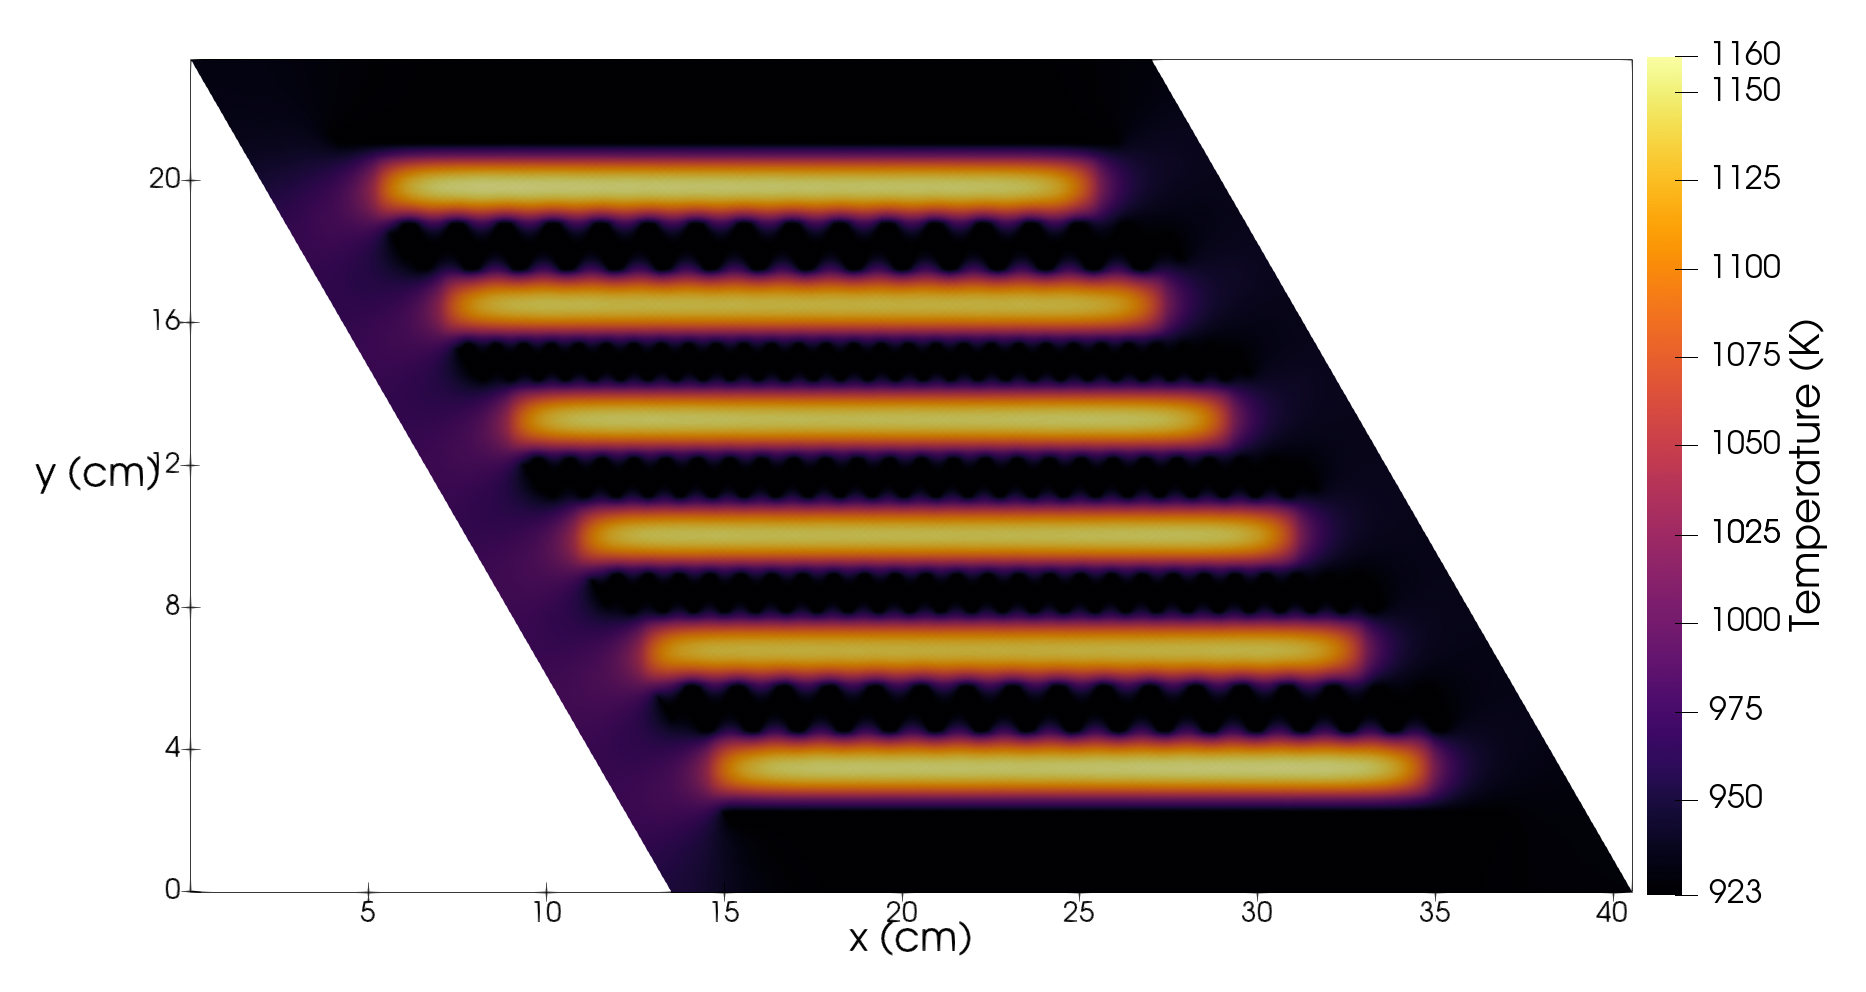
\includegraphics[width=\linewidth]{a-1e-temp-distribution-2d.png}
        \caption{2D temperature distribution.}
        \label{fig:a-1e-temp-distribution-2d} 
    \end{subfigure}
    \begin{subfigure}{\textwidth}
        \centering
        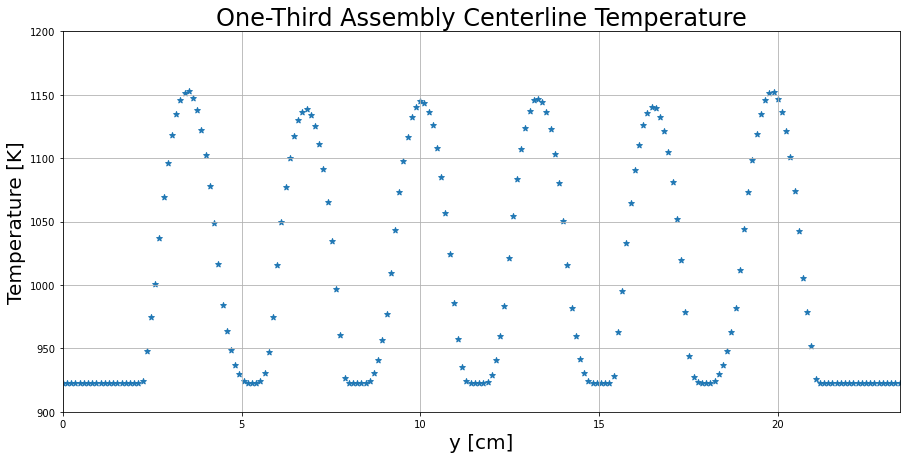
\includegraphics[width=\linewidth]{a-1e-temp-distribution-centerline.png}
        \caption{Centerline temperature. AHTR assembly's centerline is the white line 
        in Figure \ref{fig:ahtr-assem-verification}.}
        \label{fig:a-1e-temp-distribution-centerline} 
    \end{subfigure}
    \caption{Simulation a-1e's most-minimized $T_{max}$ reactor model's temperature 
    distribution.}
    \label{fig:a-1e-temp-distribution}
\end{figure}

Figure \ref{fig:a-1e-temp-distribution} demonstrates that the temperature peaks in 
top and bottom graphite planks. 
$r_1$ and $r_5$ control the coolant channel shape of the \gls{FLiBe} channels closest 
to the top and bottom graphite planks. 
To minimize maximum one-third assembly temperature, \gls{ROLLO} maximizes 
$r_1$ and $r_5$ to enable enhanced cooling in the top and bottom graphite planks. 
Thus, depending on the temperature distribution in a one-third assembly, the FLiBe 
channels (corresponding to $r_1, r_2, r_3, r_4, r_5$) closest to the temperature peaks 
will be most important to minimizing maximum one-third assembly temperature. 

\paragraph{Summary}
I verified that similar to the \gls{AHTR} plank model, the one-third assembly's 
minimize $T_{max}$ objective also flattens TRISO distribution. 
For the one-third assembly, the FLiBe channels (corresponding to $r_1, r_2, r_3, r_4, 
r_5$) closest to the temperature peaks will be most important to minimizing maximum
one-third assembly temperature, and thus, will show a negative correlation with 
$T_{max}$. 

\subsection{Discussion: Minimize $PPF_{fuel}$ Objective}
\label{sec:assem-discussion-ppf}
\paragraph{Simulation a-1c}
In Section \ref{sec:assem-1-obj-ppf}'s simulation a-1c, I conducted a single-objective 
optimization simulation to minimize fuel-normalized power peaking factor ($PPF_{fuel}$) 
by varying TRISO distribution. 
In simulation a-1c, \gls{ROLLO} found that for $PF_{total}$ = 0.06, the reactor model 
with the most-minimized $PPF_{fuel}$ has a $PPF_{fuel} = 1.0872$, an oscillating 
TRISO distribution along the x-axis, and a packing fraction standard deviation of 
$0.017$ across the one-third assembly. 

Section \ref{sec:assem-discussion-pf} concluded that for the \gls{AHTR} plank 
model, the minimize $PPF_{fuel}$ objective is driven by flattening thermal 
(Group 4) flux distribution. 
I compare the flux distributions for the most-minimized $PPF_{fuel}$ reactor model  
($PPF_{fuel} = 1.0872$) and the reactor model in simulation a-1c's final generation
with the highest $PPF_{fuel} = 1.2431$. 
Figure \ref{fig:a-1c-ppf-triso-comparison} shows the TRISO distributions for the 
compared reactor models. 
\begin{figure}[htbp!]
    \centering
    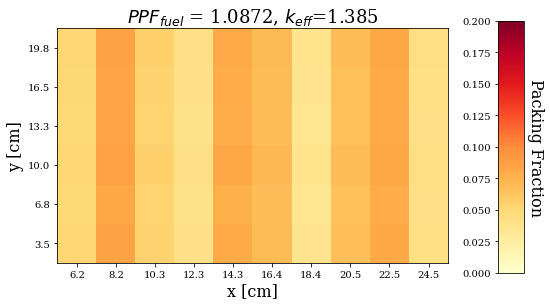
\includegraphics[width=0.49\linewidth]{a-1c-ppf-triso-comparison-most-minimized.png} 
    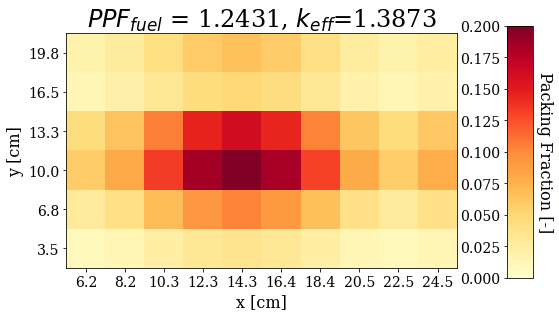
\includegraphics[width=0.49\linewidth]{a-1c-ppf-triso-comparison-least-minimized.png} 
    \caption{Simulation a-1c's most-minimized $PPF_{fuel}$ TRISO distribution 
    from Figure \ref{fig:assem-obj-1-ppf} (left) and the highest $PPF_{fuel}$ TRISO 
    distribution (right).}
    \label{fig:a-1c-ppf-triso-comparison}
\end{figure}

Figure \ref{fig:a-1c-flux-comparison} compares the 4 energy group flux distributions 
between simulation a-1c's most-minimized $PPF_{fuel}$ TRISO distribution and highest 
$PPF_{fuel}$ TRISO distribution (both distributions shown in Figure 
\ref{fig:a-1c-ppf-triso-comparison}). 
\begin{figure}[htbp!]
    \centering
    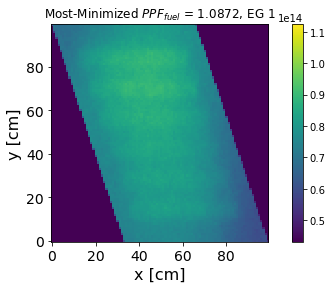
\includegraphics[width=0.35\linewidth]{flux-comparison-a-1c-most-minimized-grp1.png} 
    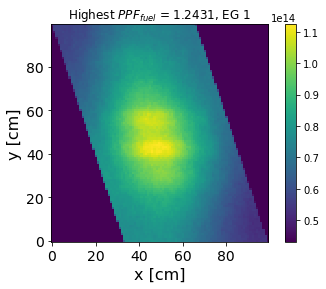
\includegraphics[width=0.35\linewidth]{flux-comparison-a-1c-least-minimized-grp1.png} 
    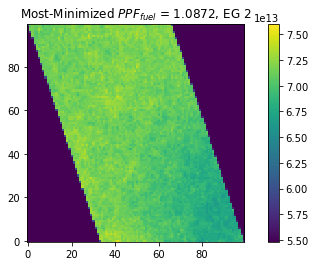
\includegraphics[width=0.35\linewidth]{flux-comparison-a-1c-most-minimized-grp2.png} 
    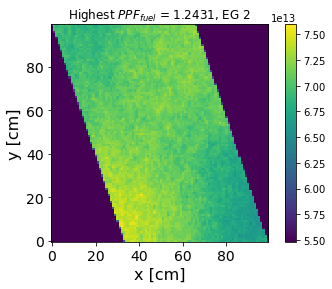
\includegraphics[width=0.35\linewidth]{flux-comparison-a-1c-least-minimized-grp2.png} 
    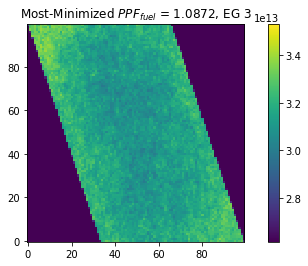
\includegraphics[width=0.35\linewidth]{flux-comparison-a-1c-most-minimized-grp3.png} 
    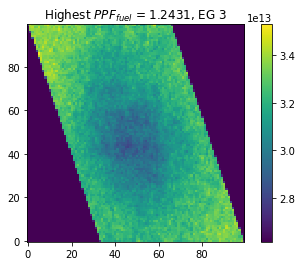
\includegraphics[width=0.35\linewidth]{flux-comparison-a-1c-least-minimized-grp3.png} 
    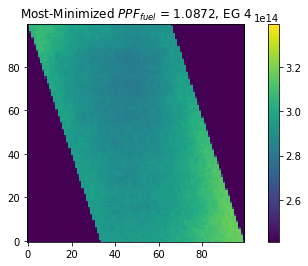
\includegraphics[width=0.35\linewidth]{flux-comparison-a-1c-most-minimized-grp4.png} 
    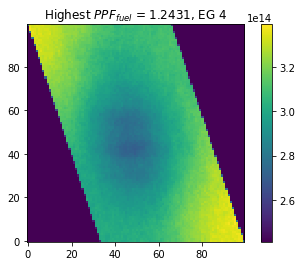
\includegraphics[width=0.35\linewidth]{flux-comparison-a-1c-least-minimized-grp4.png} 
    \caption{AHTR one-third assembly's flux comparison between the two reactor models 
    in Figure \ref{fig:a-1c-ppf-triso-comparison}: simulation a-1c's most-minimized 
    $PPF_{fuel}$ reactor model with $PPF_{fuel} = 1.0872$ and simulation a-1c's reactor 
    model with the highest $PPF_{fuel} = 1.2431$.
    Energy Group 1: E $> 9.1188 \times 10^{-3}$ MeV, 
    Energy Group 2: $2.9023 \times 10^{-5} < E < 9.1188 \times 10^{-3}$ MeV,
    Energy Group 3:  $1.8556 \times 10^{-5} < E < 2.9023 \times 10^{-5}$ MeV,
    Energy Group 4:  $1.0 \times 10^{-12} < E < 1.8554 \times 10^{-6}$ MeV.}
    \label{fig:a-1c-flux-comparison}
\end{figure}

In Figure \ref{fig:a-1c-flux-comparison}, the reactor model with the highest 
$PPF_{fuel} = 1.2431$ Group 4 flux dips in the center of the one-third assembly 
due to spatial self-shielding effects. 
In the highest $PPF_{fuel} = 1.2431$ reactor model's Group 1 flux, there is a peak in 
fast neutrons born in the one-third assembly's center, the fast neutrons are moderated 
in the graphite matrix and graphite structure (Figure \ref{fig:ahtr_assembly}). 
The self-shielding neutrons are more likely absorbed at the one-third assembly's outer 
pure graphite structure moderating regions. 
The outer areas of the one-third assembly geometrically shield the one-third assembly's 
center from neutron flux, leading to a relatively lower group 4 thermal flux in the 
center for the highest $PPF_{fuel} = 1.2431$ reactor model.

Table \ref{tab:a-1c-flux-comparison} quantifies the total flux differences per energy 
group between the compared reactor models. 
The flux values were tallied for each energy group within the one-third assembly model 
using a 100 x 100 mesh. 
% TODO: describe max and min phi, and the difference calculation. 
\begin{table}[htbp!]
    \centering
    \onehalfspacing
    \caption{Flux value comparison between the two reactor models in Figure 
    \ref{fig:a-1c-ppf-triso-comparison}: simulation a-1c's most-minimized $PPF_{fuel}$ reactor model 
    with $PPF_{fuel} = 1.0872$ and simulation a-1c's reactor model with the highest 
    $PPF_{fuel} = 1.2431$.
    Energy Group 1: E $> 9.1188 \times 10^{-3}$ MeV, 
    Energy Group 2: $2.9023 \times 10^{-5} < E < 9.1188 \times 10^{-3}$ MeV,
    Energy Group 3:  $1.8556 \times 10^{-5} < E < 2.9023 \times 10^{-5}$ MeV,
    Energy Group 4:  $1.0 \times 10^{-12} < E < 1.8554 \times 10^{-6}$ MeV.}
	\label{tab:a-1c-flux-comparison}
    \footnotesize
    \begin{tabular}{lp{4cm}p{3.3cm}p{4cm}}
    \hline
    \textbf{Energy Group} &
    \textbf{$max(\phi)/min(\phi)$ Most-minimized $PPF_{fuel}$ TRISO Distribution} & 
    \textbf{$max(\phi)/min(\phi)$ Highest $PPF_{fuel}$ TRISO Distribution} & 
    \textbf{$\%$ Difference}\\
    \hline 
    1 & 1.825 & 2.608 & \Minus30.00 \\
    2 & 1.341 & 1.386 & \Minus3.18 \\
    3 & 1.302 & 1.334 & \Minus2.43 \\
    4 & 1.319 & 1.331 & \Minus0.85 \\
    \hline
    \end{tabular}
\end{table}

In energy group 4, the most-minimized $PPF_{fuel}$ flux distribution is $0.85\%$ flatter 
than the reactor model with the highest $PPF_{fuel} = 1.2431$ (as shown by Equation 
\ref{eq:flux-prop-ppf}). 
These results verify that similar to the \gls{AHTR} plank model, the \gls{AHTR} one-third 
assembly model's minimize $PPF_{fuel}$ objective is also driven by flattening thermal 
(Group 4) flux distribution. 

\paragraph{Simulation p-1f}
In Section \ref{sec:assem-1-obj-ppf}'s simulation a-1f, I conducted a single-objective 
optimization simulation to minimize fuel-normalized power peaking factor ($PPF_{fuel}$) by 
varying coolant channel shape. 
In simulation a-1f, \gls{ROLLO} found that there is no correlation 
between $PPF_{fuel}$ and coolant channel shape (demonstrated in Figure 
\ref{fig:a-1f}). 

\paragraph{Summary}
I verified that the minimize $PPF_{fuel}$ objective for the \gls{AHTR} one-third assembly 
model is also driven by flattening thermal (Group 4) flux distribution. 
The minimize $PPF_{fuel}$ objective has correlations with the following input parameters: 
$PF_{total}$ and TRISO packing fraction distribution. 
The objective has no correlation with coolant channel shape input parameter.

\subsection{Discussion: Multi-Objective Optimization}
\label{sec:assem-discussion-multi}

\subsubsection{Simulation a-2a}
In Section \ref{sec:a-2a}'s simulation a-2a, I conducted a two-objective 
optimization simulation to minimize total fuel packing fraction ($PF_{total}$) and 
maximum temperature ($T_{max}$) in a one-third assembly model by varying total fuel 
packing fraction ($PF_{total}$) and TRISO distribution. 
In simulation a-2a, ROLLO found 13 reactor models on the Pareto Front (Figure 
\ref{fig:assem-obj-2-pftemp-pareto}). 

In simulation a-2a, \gls{ROLLO} found that the one-third assembly models with the 
most-minimized $PF_{total}$ objective, reactor models 3 and 4 (Figure 
\ref{fig:assem-obj-2-pftemp-pareto-distr}), have an oscillating TRISO distribution 
along the both the x-axis and y-axis. 
Figure \ref{fig:a-2a-pf-triso-comparison} compares simulation a-2a's reactor model 3 and 
simulation a-1a's most-minimized $PF_{total}$ reactor model. 
\begin{figure}[htbp!]
    \centering
    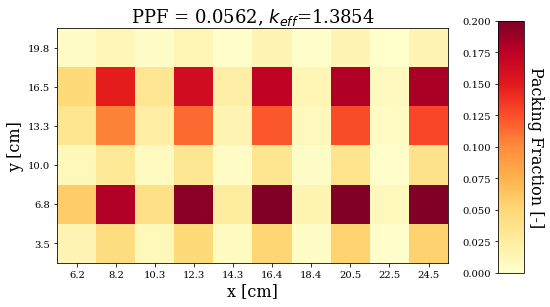
\includegraphics[width=0.49\linewidth]{a-2a-pf-most-minimized.png} 
    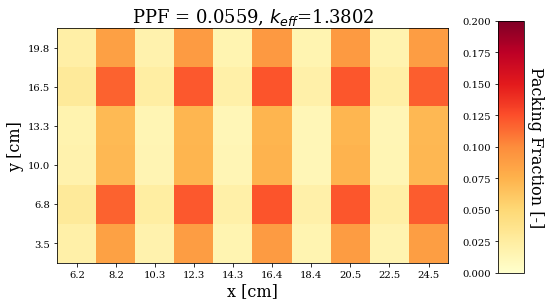
\includegraphics[width=0.49\linewidth]{assem-0.0559-most-minimized.png} 
    \caption{Simulation a-2a's most-minimized $PF_{total}$ TRISO distribution 
    from Figure \ref{fig:assem-obj-2-pftemp} (left) and simulation a-1a's 
    most-minimized $PF_{total}$ TRISO distribution from Figure 
    \ref{fig:assem-obj-1-pf} (right).}
    \label{fig:a-2a-pf-triso-comparison}
\end{figure}
Figure \ref{fig:a-2a-pf-triso-comparison} shows that simulation a-2a's most-minimized 
$PF_{total}$ reactor model and simulation a-1a's most-minimized $PF_{total}$ reactor 
model have similar distributions with peaks on the even fuel cell columns. 

In simulation a-2a, \gls{ROLLO} found that the one-third assembly model with the 
most-minimized $T_{max}$ objective, reactor model 9 (Figure 
\ref{fig:assem-obj-2-pftemp-pareto-distr}), has an almost constant TRISO distribution.
Figure \ref{fig:a-2a-temp-triso-comparison} compares simulation a-2a's reactor model 9 
and simulation a-1b's most-minimized $T_{max}$ reactor model.  
% TODO: update these figs once a-1b finishes running
\begin{figure}[htbp!]
    \centering
    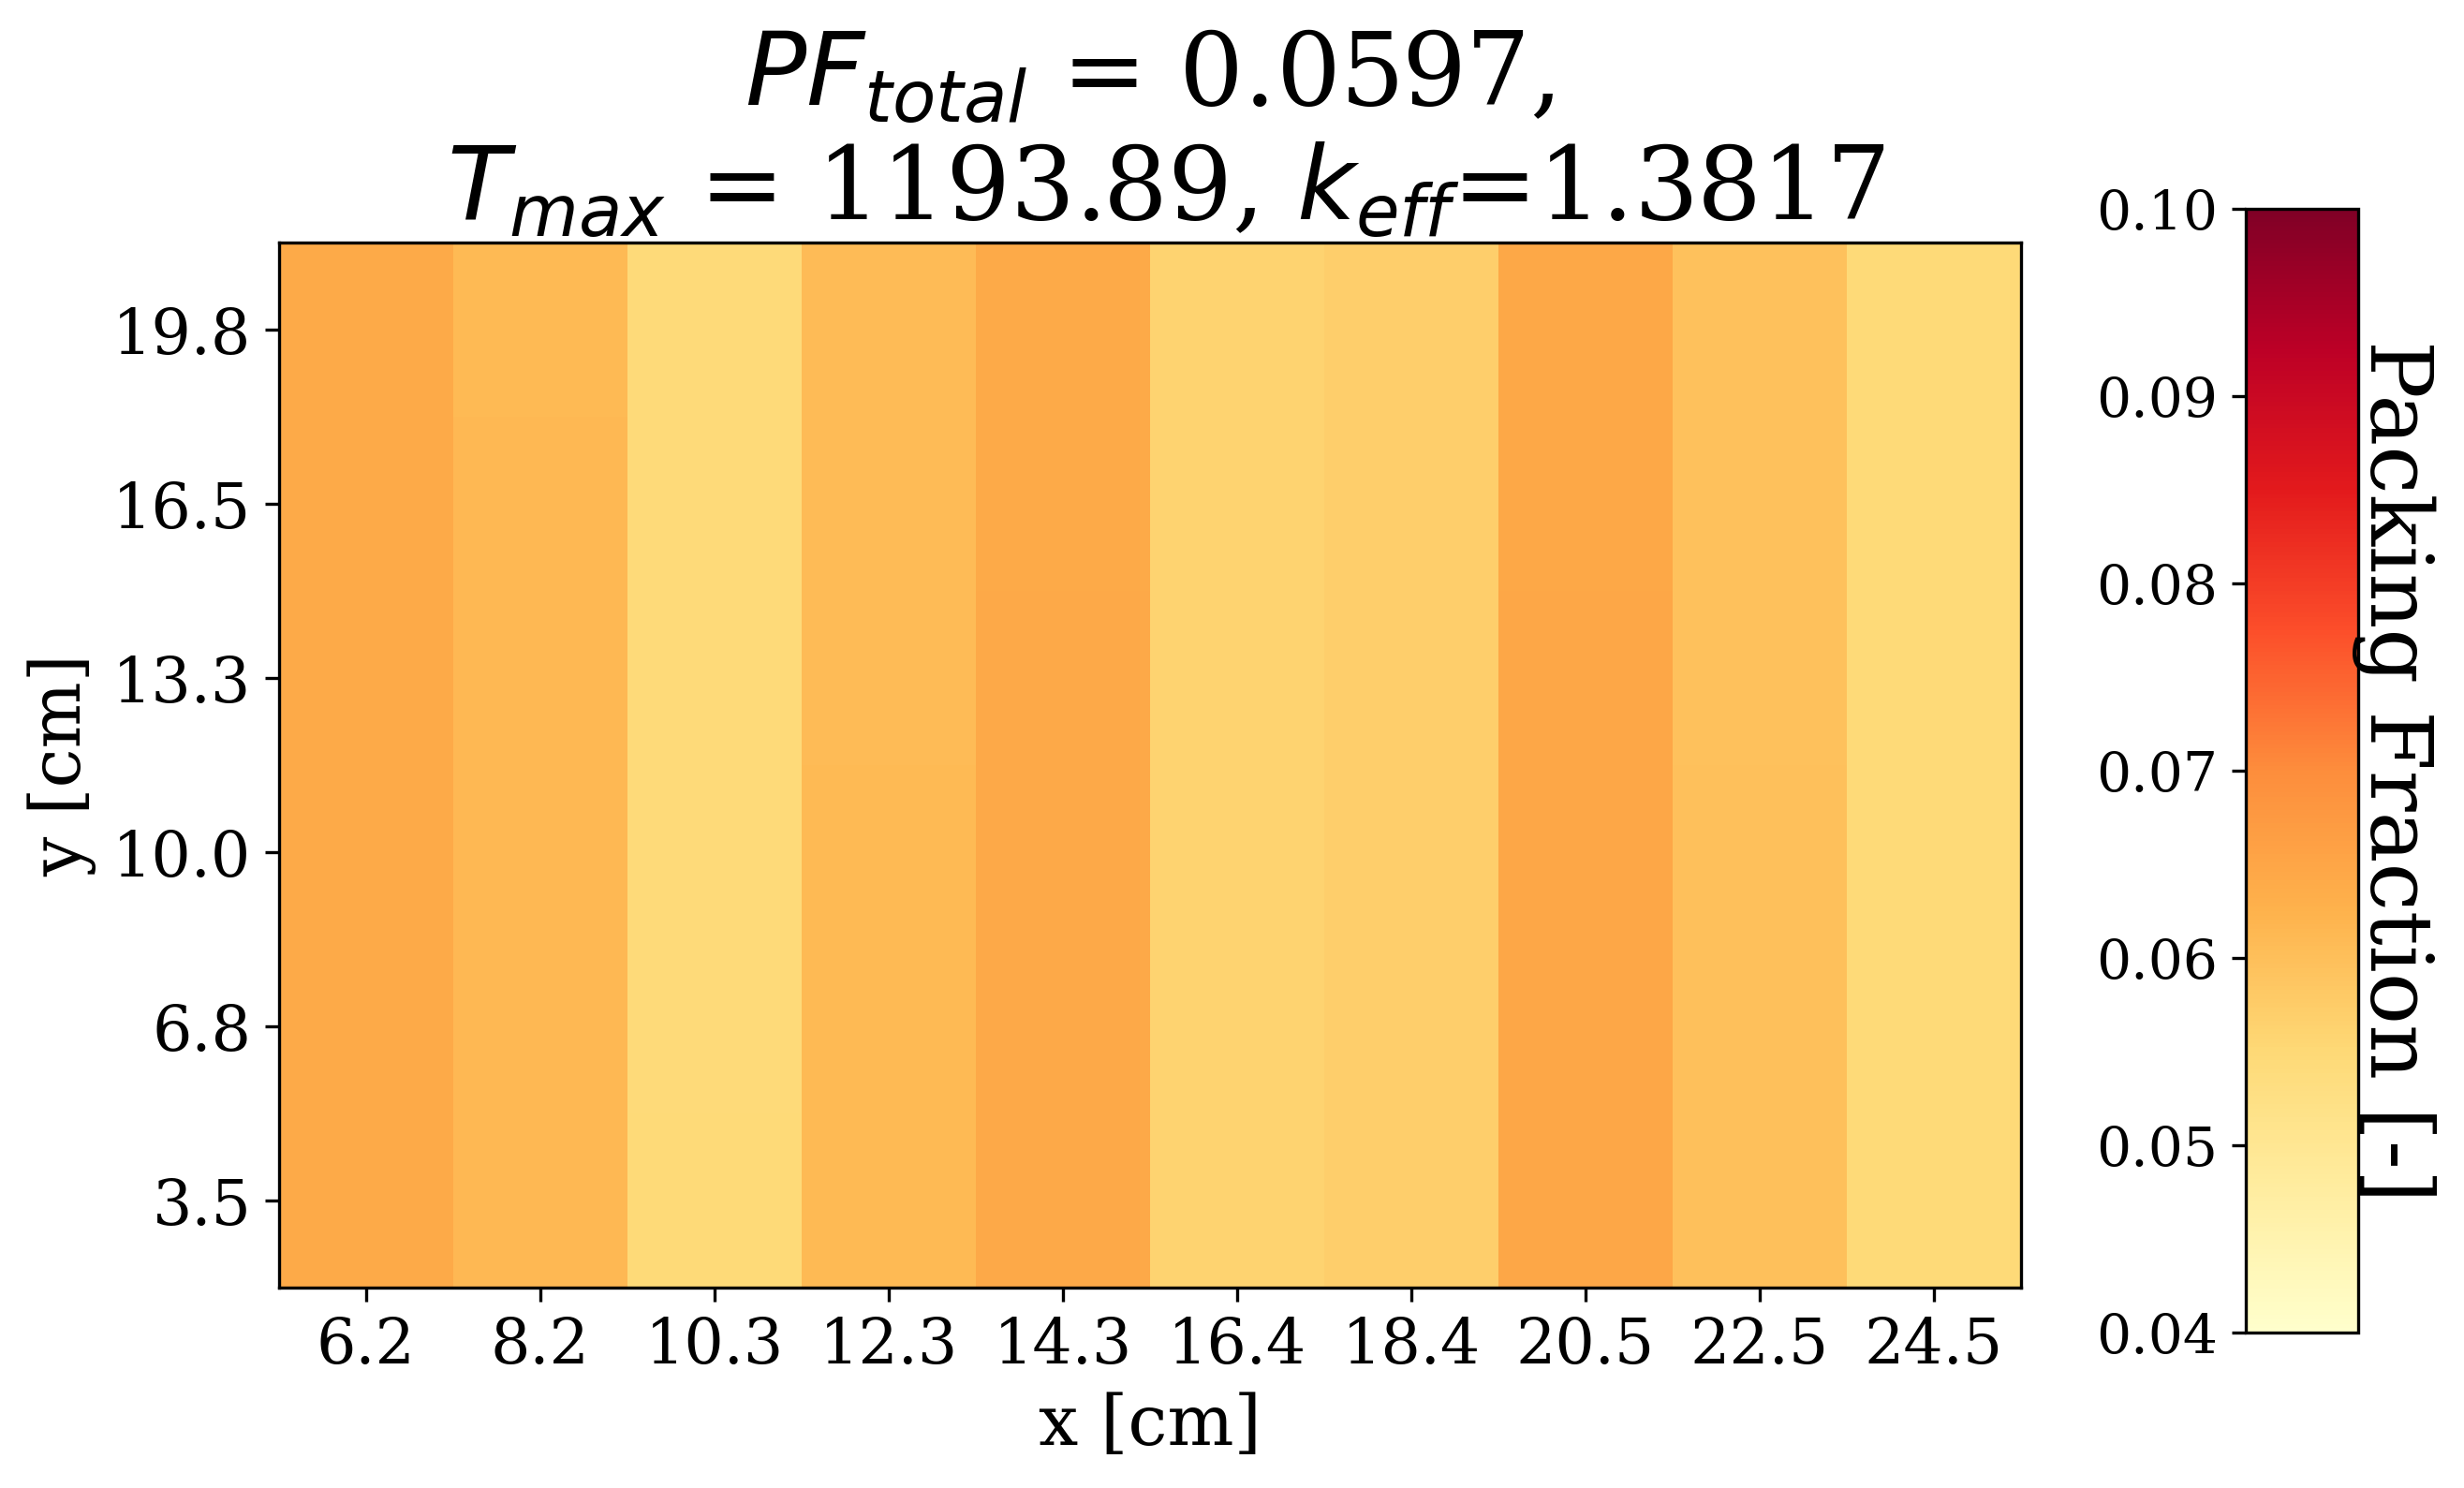
\includegraphics[width=0.49\linewidth]{a-2a-temp-most-minimized.png} 
    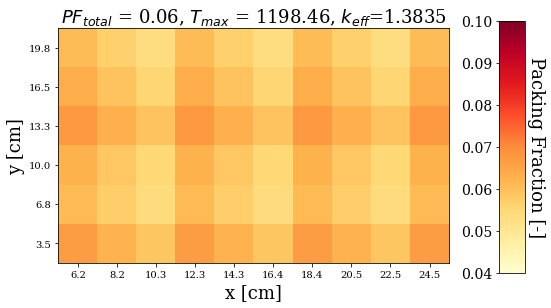
\includegraphics[width=0.49\linewidth]{a-1b-temp-most-minimized.png} 
    \caption{Simulation a-2a's most-minimized $T_{max}$ TRISO distribution 
    from Figure \ref{fig:assem-obj-2-pftemp} (left) and simulation a-1b's 
    most-minimized $T_{max}$ TRISO distribution from Figure 
    \ref{fig:assem-obj-1-temp} (right).}
    \label{fig:a-2a-temp-triso-comparison}
\end{figure}
Figure \ref{fig:a-2a-temp-triso-comparison} shows that simulation a-2a's most-minimized 
$T_{max}$ reactor model and simulation a-1b's most-minimized $T_{max}$ reactor model 
have similar almost constant TRISO distributions with packing fraction standard 
deviations of $0.003$ and $0.004$, respectively.
However, they have different $PF_{total}$ values. 
% TODO: explain the scaling and why it doesnt look flat... ?? 
 
The \gls{TRISO} distributions on simulation a-2a's Pareto front in Figure 
\ref{fig:assem-obj-2-pftemp} minimize both $PF_{total}$ and $T_{max}$, they vary
between the two extreme cases: most-minimized $PF_{total}$ and most-minimized $T_{max}$. 
Figure \ref{fig:a-2a-balanced-reactor-model} shows reactor model 13 which 
minimized both $PF_{total}$ and $T_{max}$ to an equal extent by balancing influences 
from both objectives. 
\begin{figure}[htbp!]
    \centering
    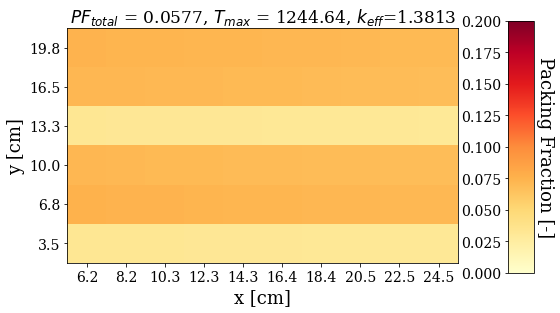
\includegraphics[width=0.7\linewidth]{a-2a-balanced-reactor-model.png} 
    \caption{Simulation a-2a's reactor model 13 which minimized both $PF_{total}$ and $T_{max}$ 
    to an equal extent (see Pareto Front in Figure \ref{fig:assem-obj-2-pftemp}).}
    \label{fig:a-2a-balanced-reactor-model}
\end{figure}
The minimize $T_{max}$ objective influences the TRISO distribution's flatness as 
described in Section \ref{sec:assem-discussion-temp}, while 
the minimize $PF_{total}$ objective influences the oscillating pattern, as described 
in Section \ref{sec:assem-discussion-pf}.

\subsubsection{Simulation a-2b}
% compare reactor models 1,3,5's fission reaction rate and thermal flux flattness
In Section \ref{sec:a-2b}'s simulation a-2b, I conducted a two-objective 
optimization simulation to minimize total fuel packing fraction ($PF_{total}$) and 
fuel-normalized power peaking factor ($PPF_{fuel}$) in a one-third assembly model 
by varying total fuel packing fraction ($PF_{total}$) and TRISO distribution. 
In simulation a-2b, ROLLO found 6 reactor models on the Pareto Front (Figure 
\ref{fig:assem-obj-2-pfppf-pareto}). 

In simulation a-2b, \gls{ROLLO} found that the one-third assembly model with the 
most-minimized $PF_{total}$ objective, reactor model 3 (Figure 
\ref{fig:assem-obj-2-pfppf-pareto-distr}), has an oscillating TRISO distribution 
along the both the x-axis and y-axis. 
Figure \ref{fig:a-2b-pf-triso-comparison} compares simulation a-2b's reactor model 3 and 
simulation a-1a's most-minimized $PF_{total}$ reactor model. 
\begin{figure}[htbp!]
    \centering
    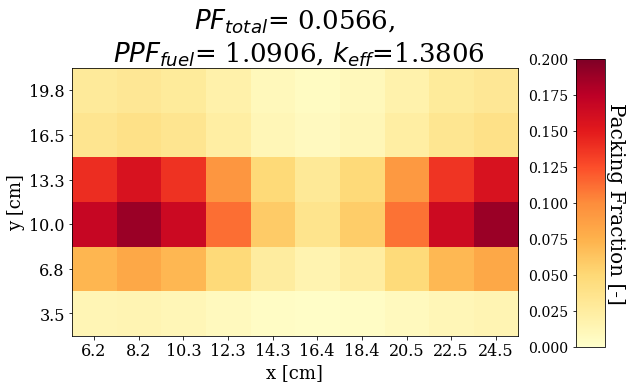
\includegraphics[width=0.49\linewidth]{a-2b-pf-most-minimized.png} 
    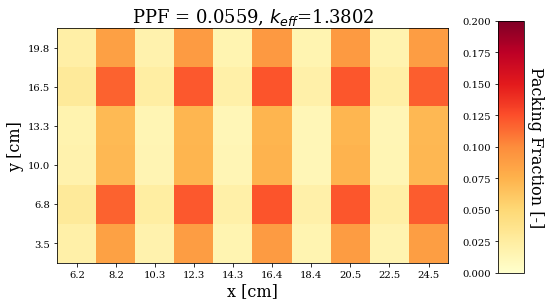
\includegraphics[width=0.49\linewidth]{assem-0.0559-most-minimized.png} 
    \caption{Simulation a-2b's most-minimized $PF_{total}$ TRISO distribution 
    from Figure \ref{fig:assem-obj-2-pfppf} (left) and simulation a-1a's 
    most-minimized $PF_{total}$ TRISO distribution from Figure 
    \ref{fig:assem-obj-1-pf} (right).}
    \label{fig:a-2b-pf-triso-comparison}
\end{figure}
Figure \ref{fig:a-2b-pf-triso-comparison} shows that simulation a-2b's reactor model 3 
and simulation a-1a's most-minimized $PF_{total}$ reactor model have similarly large 
packing fraction standard deviation of $0.032$ and $0.04$, respectively. 
However, they do not follow the same TRISO distribution pattern. 
Section \ref{sec:plank-discussion-ppf} described that in the \gls{AHTR} plank model, 
the minimize $PF_{total}$ and minimize $PPF_{fuel}$ objectives influence each other
resulting in unexpected TRISO distributions at different $PF_{total}$ values.
This explains why unlike simulation a-2a, simulation a-2b's extreme most-minimized 
$PF_{total}$ and most-minimized $PPF_{fuel}$ do not follow similar TRISO distribution 
patterns as their single-objective counterparts.
% i conduct further investigations later... 

In simulation a-2b, \gls{ROLLO} found that the one-third assembly model with the 
most-minimized $PPF_{fuel}$ objective, reactor model 1's (Figure 
\ref{fig:assem-obj-2-pfppf-pareto-distr}) TRISO distribution oscillates
along the y-axis and a oscillates slightly along the x-axis. 
Figure \ref{fig:a-2b-pf-triso-comparison} compares simulation a-2b's reactor model 1 and 
simulation a-1c's most-minimized $PPF_{fuel}$ reactor model. 
\begin{figure}[htbp!]
    \centering
    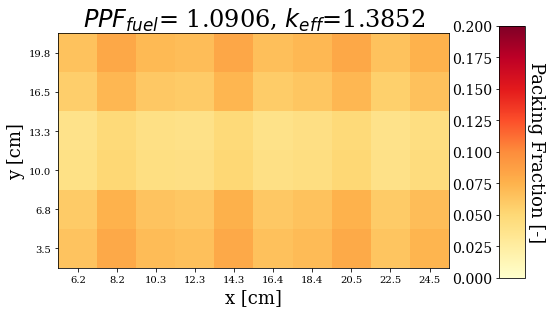
\includegraphics[width=0.49\linewidth]{a-2b-ppf-most-minimized.png} 
    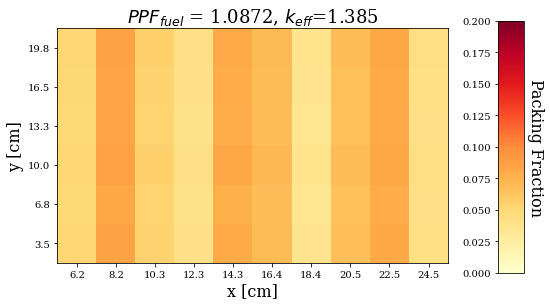
\includegraphics[width=0.49\linewidth]{a-1c-ppf-triso-comparison-most-minimized.png} 
    \caption{Simulation a-2b's most-minimized $PPF_{fuel}$ TRISO distribution 
    from Figure \ref{fig:assem-obj-2-pfppf} (left) and simulation a-1c's 
    most-minimized $PPF_{fuel}$ TRISO distribution from Figure 
    \ref{fig:assem-obj-1-ppf} (right).}
    \label{fig:a-2b-ppf-triso-comparison}
\end{figure}
Figure \ref{fig:a-2b-pf-triso-comparison} shows that simulation a-2b's reactor model 3 
and simulation a-1a's most-minimized $PF_{total}$ reactor model have similarly small 
packing fraction standard deviation of $0.013$ and $0.017$ for simulations a-2b and 
a-1c, respectively. 
However, they do not follow the same TRISO distribution pattern, this could be 
attributed to the $PF_{total}$ and $PPF_{fuel}$ relationship resulting in unexpected 
TRISO distributions at different $PF_{total}$ values, as mentioned previously. 

To better understand the driving factors for the reactor models on simulation a-2b's 
Pareto Front, I do a deep dive into the driving factors for the minimize $PF_{total}$ 
and minimize $PPF_{fuel}$ objectives. 

\paragraph{Driving Factor Quantification}
Chapter \ref{chap:ahtr-plank-opt-results} concluded that for the \gls{AHTR} plank, the 
minimize $PF_{total}$ objective is driven by maximizing the total fission reaction rate 
and the minimize $PPF_{fuel}$ objective is driven by flattening the thermal flux
distribution. 
Sections \ref{sec:assem-discussion-pf} and \ref{sec:assem-discussion-ppf} verified 
that for the \gls{AHTR} one-third assembly, the minimize $PF_{total}$ objective 
is also driven by maximizing the total fission reaction rates and the minimize 
$PPF_{fuel}$ objective is also driven by flattening the thermal flux distribution. 
This section compares the total fission reaction rate and thermal flux flatness for 
3 reactors models on simulation a-2b's Pareto Front (Figure 
\ref{fig:assem-obj-2-pfppf-pareto}): reactor model 1 with most-minimized $PPF_{fuel}$, 
reactor model 3 with most-minimized $PF_{total}$, and reactor model 5 that minimizes 
both $PF_{total}$ and $PPF_{fuel}$ to an equal extent.
Figure \ref{fig:a-2b-comparison-reactors} shows the TRISO packing fraction distribution 
for the 3 reactors models.
\begin{figure}[htbp!]
    \centering
    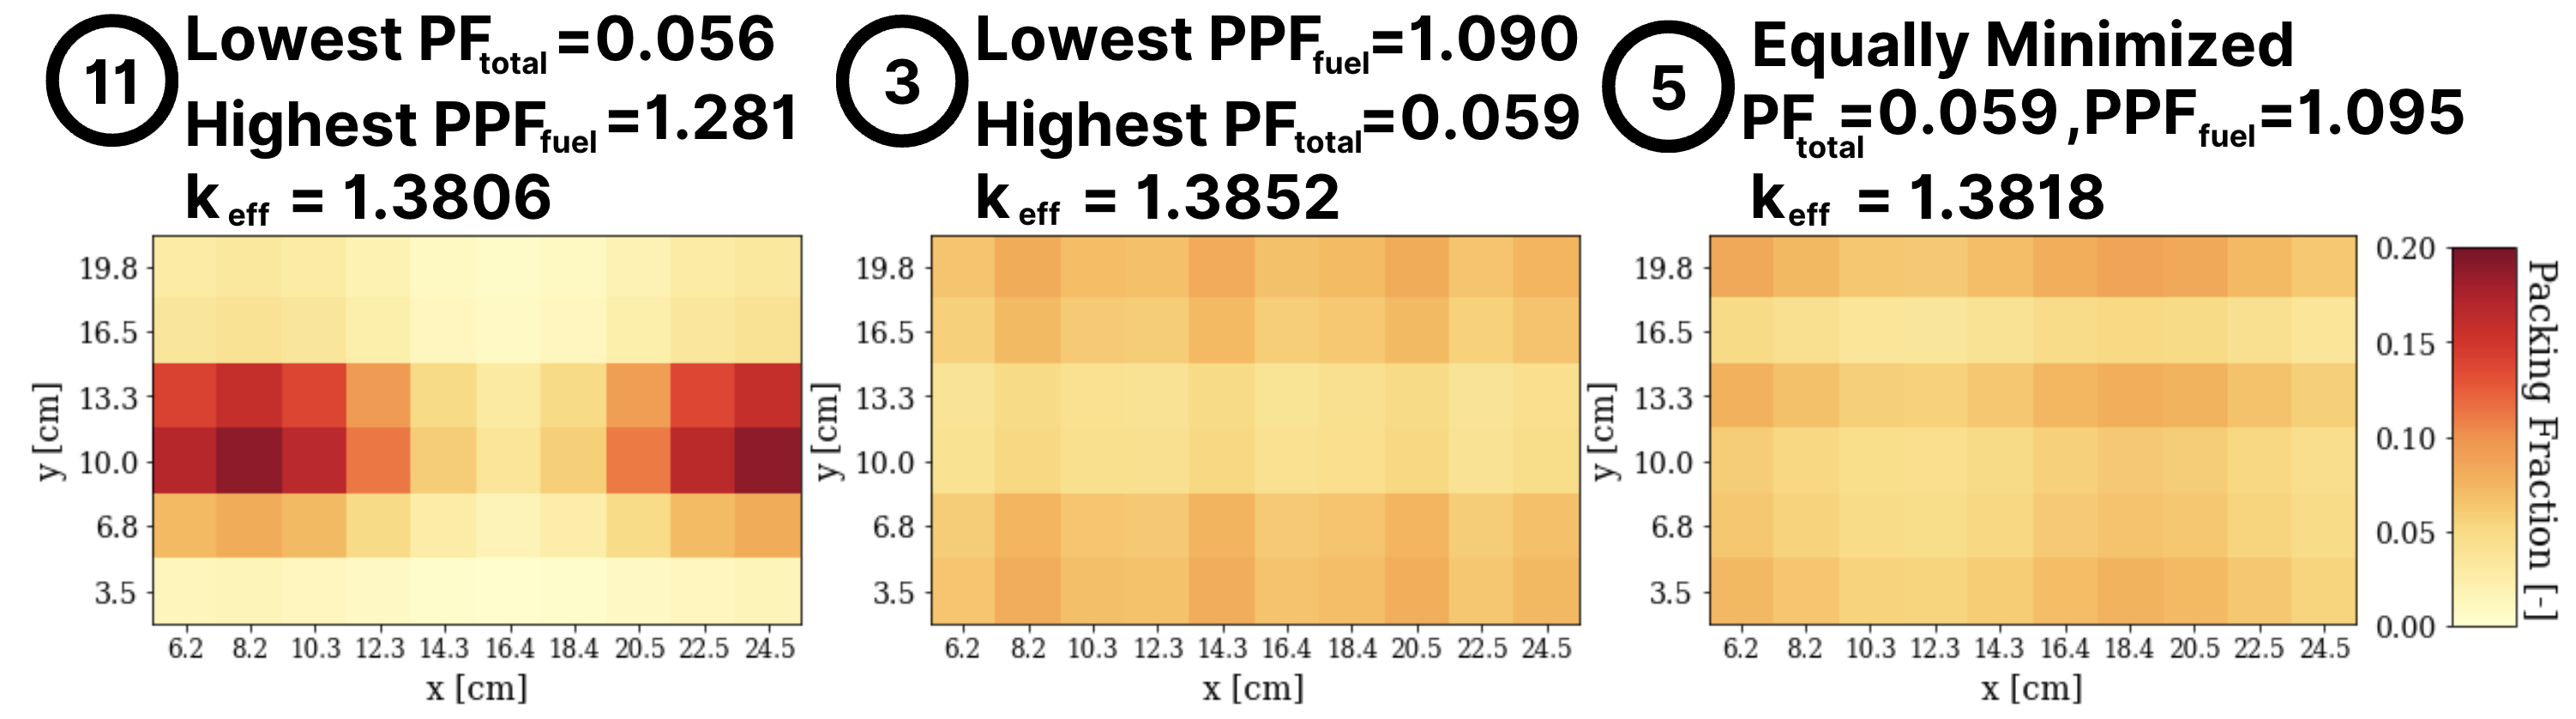
\includegraphics[width=\linewidth]{a-2b-comparison-reactors.png}  
    \caption{TRISO distributions for 3 reactor models on Simulation a-2b's Pareto Front 
    (Figure \ref{fig:assem-obj-2-pfppf-pareto}): reactor model 1 with most-minimized 
    $PPF_{fuel}$ (left), reactor model 3 with most-minimized $PF_{total}$ (middle), 
    and reactor model 5 that minimizes both $PF_{total}$ and $PPF_{fuel}$ to an equal 
    extent (right).}
    \label{fig:a-2b-comparison-reactors}
\end{figure}

Table \ref{tab:a-2b-comparison-reactors} shows the $PF_{total}$, $PPF_{fuel}$, TRISO 
packing fraction standard deviation, total fission reaction rate, and thermal flux 
flatness for the three reactor models. 
\begin{table}[htbp!]
    \centering
    \onehalfspacing
    \caption{$PF_{total}$, $PPF_{fuel}$, TRISO packing fraction distribution variance, 
    total fission reaction rate, and thermal flux flatness for 3 reactor models on Simulation 
    a-2b's Pareto Front (Figure \ref{fig:assem-obj-2-pfppf-pareto}): reactor model 1 with 
    most-minimized $PPF_{fuel}$, reactor model 3 with most-minimized $PF_{total}$, 
    and reactor model 5 that minimizes both $PF_{total}$ and $PPF_{fuel}$ to an equal extent.}
	\label{tab:a-2b-comparison-reactors}
    \footnotesize
    \begin{tabular}{p{2.9cm}p{1.5cm}p{2cm}p{2.3cm}lp{2.5cm}l}
    \hline
    \textbf{Most Minimized Param} & \textbf{Reactor Model} 
    & \textbf{TRISO Distr SD} & \textbf{Fission Rxn Rate} & \textbf{$\%$ Diff}
    & $max(\phi_4)/min(\phi_4)$ & \textbf{$\%$ Diff}\\
    \hline 
    \textbf{Both} & 5 & 0.003 & 0.5472 & - & 1.2897 & -\\
    \textbf{$PF_{total}$} & 3 & 0.024 & 0.5476 & \Plus0.07 & 1.2949 & \Plus0.40\\
    \textbf{$PPF_{fuel}$} & 1 & 0.003 & 0.5478 & \Plus0.12 & 1.2851 & \Minus0.35\\
    \hline
    \end{tabular}
\end{table}

The most minimized $PF_{fuel}$ reactor model 1 has the highest fission reaction rate, 
followed by the most minimized $PF_{fuel}$ reactor model 3, and then reactor model 5 that 
minimizes both $PF_{total}$ and $PPF_{fuel}$ to an equal extent.
Reactor model 3 has a higher fission reaction rate compared to reactor model 5 despite 
reactor model 3 having a lower $PF_{total}$.
Reactor model 3's oscillating TRISO distribution enables a higher fission reaction rate, 
and thus, 240pcm higher $k_{eff}$ for a lower $PF_{total}$ compared to reactor model 5. 

The most minimized $PPF_{fuel}$ reactor model 1 has the flattest thermal flux, followed by 
reactor model 5 that minimizes both $PF_{total}$ and $PPF_{fuel}$ to an equal extent, and 
then the most minimized $PF_{fuel}$ reactor model 3. 
Section \ref{sec:assem-discussion-ppf} verified that the \gls{AHTR} one-third assembly model's 
minimize $PPF_{fuel}$ objective is also driven by flattening thermal (Group 4) flux 
distribution. 
Therefore, explaining why the most minimized $PPF_{fuel}$ reactor model 1 has the 
flattest thermal flux distribution. 

% comment on how the high TRISO variance results in less flat flux. constrasting objectives

\subsubsection{Simulation a-2c}
In Section \ref{sec:a-2c}'s simulation a-2c, I conducted a two-objective 
optimization simulation to minimize maximum temperature ($T_{max}$) and fuel-normalized 
power peaking factor ($PPF_{fuel}$) in a one-third assembly model by varying 
TRISO distribution. 
In simulation a-2c, ROLLO found 1 reactor model on the Pareto Front (Figure 
\ref{fig:assem-obj-2-tempppf-pareto}), demonstrating that minimize $T_{max}$ and 
minimize $PPF_{fuel}$ objectives are non-contrasting for the one-third assembly model. 

Figure \ref{fig:a-2c-triso-comparison} compares the single reactor model on simulation 
a-2c's Pareto Front, simulation a-1b's most-minimized $T_{max}$ reactor model, and 
simulation a-1c's most-minimized $PPF_{fuel}$ reactor model. 
All reactor models have $PF_{total}=0.06$.
\begin{figure}[htbp!]
    \centering
    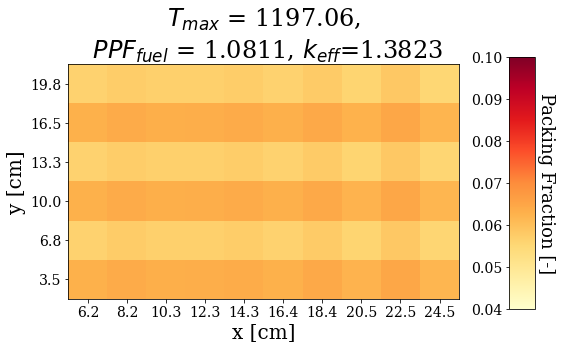
\includegraphics[width=0.51\linewidth]{a-2c-most-minimized.png} 
    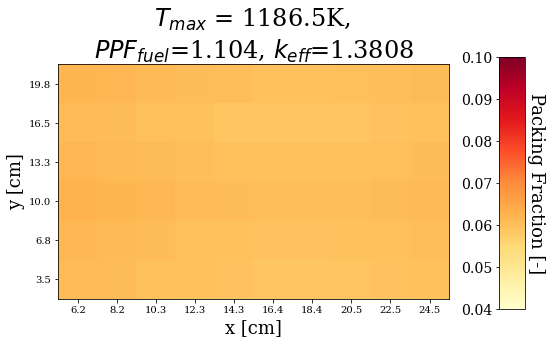
\includegraphics[width=0.49\linewidth]{a-1b-temp-most-minimized-with-ppf.png} 
    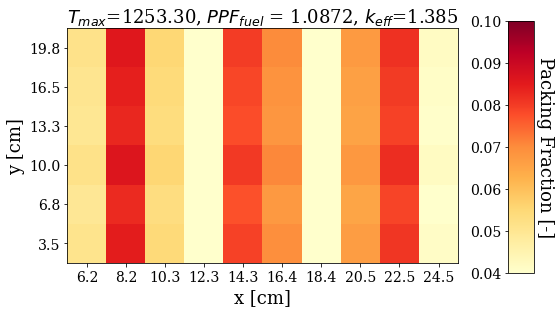
\includegraphics[width=0.49\linewidth]{a-1c-ppf-triso-comparison-most-minimized-01-scale.png} 
    \caption{Simulation a-2c's single Pareto Front reactor model's TRISO distribution 
    from Figure \ref{fig:assem-obj-2-tempppf} (above), simulation a-1b's most-minimized 
    $T_{max}$ TRISO distribution from Figure \ref{fig:assem-obj-1-temp} (lower left), and 
    simulation a-1c's most-minimized $PPF_{fuel}$ TRISO distribution from Figure 
    \ref{fig:assem-obj-1-ppf} (lower right).
    All reactor models have $PF_{total}=0.06$.}
    \label{fig:a-2c-triso-comparison}
\end{figure}

Figure \ref{fig:a-2c-triso-comparison} shows that the single reactor model on simulation 
a-2c's Pareto Front's TRISO distributions is more similar to simulation a-1b's 
most-minimized $T_{max}$ TRISO distribution than simulation a-1c's most-minimized 
$PPF_{fuel}$ TRISO distribution. 
Simulation a-1c's most-minimized $PPF_{fuel}$ reactor model has a high $T_{max}=1253.30$, 
while simulation a-1b's most-minimized $T_{max}$ reactor model has a low 
$PPF_{fuel}=1.104$. 
Therefore, influences from the minimize $T_{max}$ objective, results in the single 
reactor model on simulation a-2c's Pareto Front to have a TRISO distribution more 
similar to simulation a-1b's most-minimized $T_{max}$ reactor model. 

% add PPF values.. 
% comment... 
%a-2c: $0.0033$
%a-1b: $0.004$
%a-1c: $0.017$

\subsubsection{Simulation a-3a}
In Section \ref{sec:a-3a}'s simulation a-3a, I conducted a three-objective 
optimization simulation to minimize total fuel packing fraction ($PF_{total}$), 
maximum temperature ($T_{max}$), and fuel-normalized power peaking factor 
($PPF_{fuel}$) in a one-third assembly model by varying $PF_{total}$ and 
TRISO distribution.
\gls{ROLLO} found xx widely spread reactor models on simulation a-3a's Pareto 
front (Figure xx). 

\subsubsection{Simulation a-3b}
In Section \ref{sec:a-3b}'s simulation a-3b, I conducted a three-objective 
optimization simulation to minimize total fuel packing fraction ($PF_{total}$), 
maximum temperature ($T_{max}$), and fuel-normalized power peaking factor 
($PPF_{fuel}$) in a one-third assembly model by varying $PF_{total}$, 
TRISO distribution, and coolant channel shape ($r_1, r_2, r_3, r_4, r_5$).
\gls{ROLLO} found xx widely spread reactor models on simulation a-3b's Pareto 
front (Figure xx). 

\subsection{Discussion: Major Takeaways}

\section{Summary}

% talk about p-3b result, what is recommended for the AHTR assembly's geometry. 